\chapter{System Design}
\label{chapter:design}

\section{Overview}

\begin{figure}[hb]
    \centering
    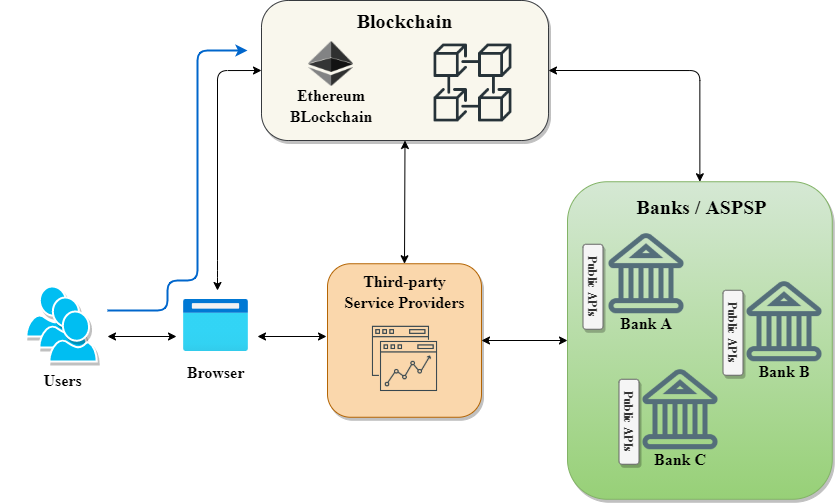
\includegraphics[height=!,width=1\linewidth,keepaspectratio=true]{figures/system architecture-banks.png}
    \caption{{\footnotesize System Architecture}}
    \label{fig:system_architecture}
\end{figure}

    In our system prototype, we have three roles, including customer (user), financial institution, and third-party services provider. Figure~\ref{fig:system_architecture} shows the relation between these roles. Each customer iteracts with Blockchain by using MetaMask, they not only login with MetaMask but also manage their own access manager contract.

\section{Scenario}

    For user perspective, our proposed system provide a single digital ID with Ethereum blockchain.

\section{Workflow}
\begin{itemize}
    \item Verify unique ID stage
    \item Binding account stage
    \item Third party login stage
\end{itemize}
\subsection{Identity verification}
\subsection{Account binding}
\subsection{Third-party login with Ethereum account}
\subsection{Data sharing}